\textbf{{1.请求分页原理}}\\

a.
基本概念:\textbf{在分页存储管理系统的基础上,增加请求调页功能、页面置换功能所形成的一种虚拟存储系统。}在请求分页存储管理中,作业运行之前,只要\textbf{将当前需要的一部分页面装入主存,便可以启动作业运行。}在作业运行过程中,若所要访问的页面不在主存中,则通过调页功能将其调入,同时还可以通过置换功能将暂时不用的页面置换到外存上,以便腾出内存空间。

{{b. 理解方式:}请求分页=基本分页+请求调页功能+页面置换功能。}

\textbf{{2.页表结构}}\\

扩充后的页表项如下图所示。

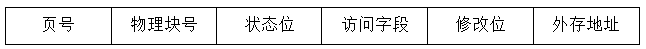
\includegraphics[width=3.33333in,height=0.25000in]{png-jpeg-pics/27CA7AD5C5B3164778806183FB4A0D06.png}

a.
页号和物理块号:其在分页存储管理中已经定义过,这两个信息是进行地址变换所必需的;\\
b. 状态位(存在位):用于判断页面是否在主存中;\\
c.
访问字段:用于记录页面在一段时间内被访问的次数,或最近已有多久未被访问,以供置换算法在选择换出页面时参考;\\
d. 修改位:用于表示页面调入内存后是否被修改过;\\
e. 外存地址:用于指出页面在外存上的存放地址,供调入页面时使用。

\textbf{{3.缺页中断与地址变换}}

a. 流程图:如下图所示。~

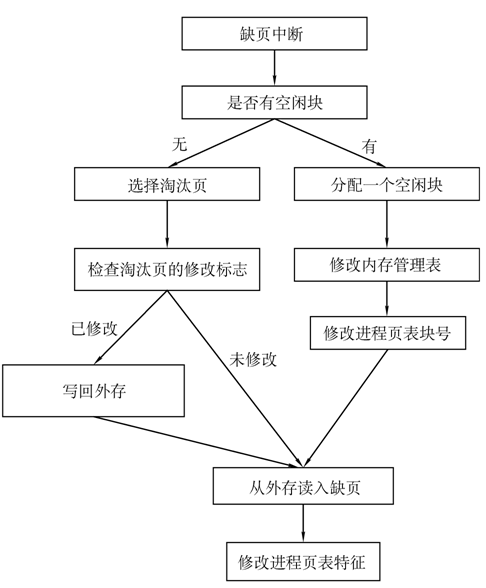
\includegraphics[width=3.12500in,height=3.78125in]{png-jpeg-pics/7A06B8CD61CF71DE38B4A51F2AC07589.png}

b.
缺页中断与一般中断的区别:在指令的执行期间产生和处理缺页中断;一条指令可以产生多个缺页中断。

\textbf{{4.请求分页管理方式的优缺点}}\\
a. 优点:\\
① 可以离散储存程序,降低了碎片数量;\\
② 提供虚拟存储器,提高了主存利用率,有利于多道程序运行,方便用户。\\
b. 缺点:\\
①必须有硬件支持;\\
②有些情况下系统会产生抖动现象;\\
③程序最后一页仍然存在未被利用的部分空间。
